\chapter{Introduction}
\renewcommand{\baselinestretch}{\mystretch}
\label{chap:Intro}
%\setlength{\parindent}{0pt}

\section{Background}

\PARstart{M}{aterial} extrusion 3D printing develops rapidly in these years. In detail, the most popular and low-cost 3D printing technology is fused deposition modelling (FDM), which is also identified as fused filament fabrication (FFF). This printing technology is based on extrusion and fused fibre material deposition. The very common material utilised in FDM technology is acrylonitrile butadiene styrene (ABS), followed by polylactic acid (PLA), polycarbonate (PC), Polyphenylsulfone (PPSF) and the mixtures. However, the lack of the variety of thermoplastics limits the utility of FDM systems. \\
\\
With the development of the extruder and the 3D printer, the limitation of the printable materials decreases. Meanwhile, the normally used polymer such as ABS is a good matrix material to combine with other materials creatively. In fact, it is common for 3D printer users to recycle 3D production and extrude a 3D print filament using different polymer blends. It is obviously regarded as a low cost and environment-friendly manufacturing. \\
\\
On the other hand, space exploration has developed to some level which there is a significant demand for tool construction in the space \cite{khoshnevis2015selective}. From a sustainable and developmental perspective, the utilisation of the Lunar and Mars regolith (powder) as the printing materials could reduce the mass of polymers we need take from the earth. Therefore, 3D printing offers a possibility of facilitating Lunar and Mars settlement with reduced logistics from the earth.

\section{The Objective of Project}
This project aims to demonstrate that useful microwave components can be 3D-printed by using Lunar and/or Mars dust simulants. As 3D printer based on FDM technology was successfully applied in low gravity space, the candidate filament was manufactured by the composite of the powdered regolith simulants and ABS pellets in this project. The very fine pumice powder was chosen as the lunar and martian regolith simulants. Particularly, the 3D printed air-filled metal-pipe rectangular waveguide as Figure \ref{Fig:waveguide} presents was investigated to verify the printing properties of these materials made by ABS and very fine pumice powder. In a word, the study presented here offers the potential of the low-cost manufacturing technology in space.\\
\begin{figure}[htbp]
  \centering
  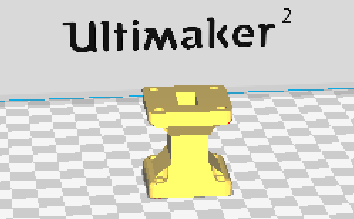
\includegraphics[scale=1.2]{Figs//waveguide_design.PNG}
  \caption[The waveguide design in Cura]{\footnotesize The waveguide design in Cura.}
  \label{Fig:waveguide}
\end{figure}
\\
More importantly, the filament samples containing different proportions of pumice was investigated to check the limitation and the influence of pumice for 3D printing, including reliable printing speed, build platform adhesion, the extruding temperature and geometrical accuracy of prints. 

\section{Thesis Outline}

The remainder of this thesis is structured as follows:
\begin{itemize}
\item Chapter Two describes the literature review of 3D printing systems, materials and the well-down research of 3D printing in the space.
\end{itemize}
\begin{itemize}
\item In Chapter Three and Four, it is shown that the actual experiments on filament production of ABS and pumice. The principle we complied with and findings when working with extruder and controller would be mentioned in detail.
\end{itemize}

\begin{itemize}
\item The investigation of the printing properties of filament is presented in Chapter Five.
\end{itemize}

\begin{itemize}
\item  At last, Chapter Six contains the conclusion of this project.
\end{itemize}


